\documentclass[11pt,a4paper]{article}

\usepackage[utf8]{inputenc}
\usepackage[T1]{fontenc}
\usepackage[margin=2.4cm]{geometry}
\usepackage{amsmath,amssymb,amsthm,bm}
\usepackage{graphicx}
\usepackage{booktabs}
\usepackage{xcolor}
\usepackage{tikz}
\usetikzlibrary{arrows.meta,positioning,decorations.pathmorphing}
\usepackage[colorlinks=true,linkcolor=NavyBlue,citecolor=NavyBlue,urlcolor=NavyBlue]{hyperref}
\definecolor{NavyBlue}{RGB}{27,73,101}
\usepackage{caption}
\captionsetup{font=small,labelfont=bf}
\usepackage{enumitem}
\setlist{itemsep=1pt,topsep=3pt}
\usepackage{titlesec}
\titleformat{\section}{\normalfont\large\bfseries}{\thesection}{0.7em}{}
\titleformat{\subsection}{\normalfont\normalsize\bfseries}{\thesubsection}{0.7em}{}

\setlength{\emergencystretch}{2.5em}

\newcommand{\dg}{^{\dagger}}
\newcommand{\Om}{\Omega}
\newcommand{\Omu}{\Omega_{\mu}}
\newcommand{\wt}{\tilde{\omega}_{0}}
\newcommand{\lc}{\lambda_{c}}
\newcommand{\ket}[1]{\lvert #1 \rangle}
\newcommand{\bra}[1]{\langle #1 \rvert}
\newcommand{\avg}[1]{\langle #1 \rangle}


\title{\bfseries Critical Dicke electrometry:\\[2pt]
\large extending intracavity Rydberg-EIT microwave sensing\\
into the superradiant phase transition}
\author{Feasibility study and literature assessment}
\date{\today}

\begin{document}
\maketitle

\begin{abstract}
\noindent
Peng \emph{et al.} [J.\ Opt.\ Soc.\ Am.\ B \textbf{35}, 2272 (2018)] showed that placing a
four-level Rydberg-EIT medium inside an optical cavity sharpens the Autler--Townes
readout of a microwave electric field. Zhang \emph{et al.} [Phys.\ Rev.\ Lett.\ \textbf{110},
090402 (2013)] showed that Rydberg polaritons in a cavity realise a generalised Dicke model
whose competition between atomic interaction and atom--light coupling produces a
superradiant solid. This note works out what happens when the two are combined \emph{and
the transition itself is used as the sensing element}: the microwave
field to be measured sets the dressed-polariton splitting $\wt$, and therefore moves the
Dicke critical coupling $\lc = \tfrac12\sqrt{\omega\wt}$. We construct the effective
Hamiltonian, identify three distinct read-out protocols, and evaluate them with exact
diagonalisation (closed system, $N\le512$) and linearised quantum Langevin theory (open,
driven system).

\medskip\noindent
The headline results are mixed, and deliberately so. \textbf{(i)} The mechanism is real and
the numbers are attractive: the ground-state quantum Fisher information scales as
$N^{4/3}$ at criticality (fitted exponent $1.307$), the driven system provides a
transduction gain $\propto\varepsilon^{-1}$ in the distance $\varepsilon=1-\lambda/\lc$ from
threshold, up to $10$~dB of intrinsic output squeezing, and a quantum-noise-limited
sensitivity of $0.18~\mathrm{nV\,cm^{-1}Hz^{-1/2}}$ at a modest collective excitation
$n_b=10^{4}$ --- an order of magnitude below the best published Rydberg electrometers.
\textbf{(ii)} But a control calculation at \emph{fixed} collective excitation shows that the
input-referred sensitivity is set entirely by $n_b$ and the atomic decoherence rate
$\gamma$, obeying $\sqrt{S_{\wt}} = 0.72\sqrt{\gamma/n_b}$ independently of how close to
threshold one sits. Criticality supplies gain and squeezing, not a new scaling law; the
$N^{4/3}$ advantage is a static-protocol artefact that critical slowing down removes, in
agreement with the known no-go results. \textbf{(iii)} We identify one genuinely novel and
defensible contribution: a \emph{null} (threshold-crossing) electrometry protocol in which
the measurand is read out as the two-photon laser detuning required to hold the system at
threshold, with the same SI traceability as Autler--Townes but a discriminant whose
sharpness is set by the transition rather than by the EIT linewidth.

\medskip\noindent
Verdict: worth pursuing, but as a \emph{critical-Dicke superheterodyne amplifier} rather than
as a claimed route to super-classical scaling, and the write-up should say so.
\end{abstract}

\tableofcontents

\section{What is being proposed}

The idea, stated compactly: take the intracavity Rydberg-EIT microwave electrometer of
Peng \emph{et al.}~\cite{Peng2018}, push it into the regime where the atom--cavity system is
described by a Dicke model with a superradiant phase transition (as in the
Rydberg-polariton setting of Zhang \emph{et al.}~\cite{Zhang2013}), and use the transition
itself --- rather than a spectroscopic line splitting --- as the microwave-field sensor.

The mechanism that makes this more than an analogy is a simple one. In the four-level ladder
$\ket{g}\!\to\!\ket{e}\!\to\!\ket{r}\!\to\!\ket{r'}$, the microwave field dresses the two
Rydberg states and thereby fixes the transition frequency $\wt$ of the effective two-level
system that the cavity mode sees. The Dicke critical coupling depends on exactly that
frequency,
\begin{equation}
  \lc = \tfrac12\sqrt{\omega\,\wt}, \qquad \wt = \delta + \Omu/2, \qquad \Omu = dE_\mu/\hbar,
  \label{eq:key}
\end{equation}
so \emph{the phase boundary is a function of the field to be measured}. Biasing the system
just below threshold turns a weak microwave field into a large, directly detected optical
signal.

Section~\ref{sec:model} builds this Hamiltonian, Sec.~\ref{sec:protocols} lays out three
protocols it supports, Sec.~\ref{sec:metrology} evaluates them numerically,
Sec.~\ref{sec:ising} adds the Rydberg interactions that make the link to
Ref.~\cite{Zhang2013} explicit, Sec.~\ref{sec:prior} reviews what has already been done, and
Sec.~\ref{sec:verdict} gives an honest assessment.

\paragraph{A note on sourcing.} The primary sources for every claim of the form ``paper X
does not do Y'' in Sec.~\ref{sec:prior} have been read first-hand: Refs.~\cite{Peng2018,
Yang2020, Wang2023} (abstracts and stated results), and Refs.~\cite{Zhang2013, Ding2022,
Wang2025} in full. Where a statement rests only on an abstract it is marked as such. The
one substantive correction this produced is recorded in Sec.~\ref{sec:ising}: the model of
Ref.~\cite{Zhang2013} is written in the rotating-wave approximation, so its transition is
not the $\mathbb{Z}_2$ superradiant transition used here.

\section{The model}
\label{sec:model}

\subsection{Level scheme and the dressed sensor spin}

Take the standard Rydberg-EIT electrometry ladder in $^{87}$Rb:
$\ket{g}=\ket{5S_{1/2}}$, $\ket{e}=\ket{5P_{3/2}}$, $\ket{r}=\ket{53D_{5/2}}$,
$\ket{r'}=\ket{54P_{3/2}}$. A probe field addresses $\ket{g}\!\to\!\ket{e}$, a strong
control laser $\Om_c$ drives $\ket{e}\!\to\!\ket{r}$, and the microwave field to be measured
drives $\ket{r}\!\to\!\ket{r'}$ with Rabi frequency $\Omu = dE_\mu/\hbar$. For this
transition $d = 1774.82\,ea_0$, giving the conversion
\begin{equation}
  \Omu/2\pi = 2.271~\mathrm{MHz} \times \left(E_\mu / \mathrm{mV\,cm^{-1}}\right).
\end{equation}
On microwave resonance the Rydberg pair is dressed into
$\ket{\pm} = (\ket{r}\pm\ket{r'})/\sqrt2$ at energies $\pm\Omu/2$: this is the
Autler--Townes doublet that conventional electrometry reads out as a line splitting. The
key move here is to treat one dressed state, say $\ket{+}$, together with $\ket{g}$ as a
single effective spin-$\tfrac12$ whose splitting is
\begin{equation}
  \wt = \delta + \Omu/2,
\end{equation}
$\delta$ being the two-photon detuning of the optical fields. \emph{The measurand has become
a Hamiltonian parameter of a two-level system}, not a spectroscopic feature to be resolved.

\subsection{Engineering the Dicke coupling}

A bare dipole coupling cannot produce a superradiant transition: the $A^2$ term and the
Thomas--Reiche--Kuhn sum rule forbid it~\cite{Rzazewski1975,Nataf2010}. The standard way
around this is the cavity-assisted Raman scheme of Dimer, Estienne, Parkins and
Carmichael~\cite{Dimer2007}, realised experimentally by Baden \emph{et
al.}~\cite{Baden2014}: two Raman channels, driven by two control fields with different
detunings, generate co-rotating and counter-rotating cavity--atom couplings
$\lambda_{1,2}$ that can be tuned independently. Here this is natural rather than
contrived, because the Rydberg-EIT ladder already \emph{is} a Raman configuration; the
second control field is the only addition. Reference~\cite{Zhang2013} makes the same point
in its own setting: because $\ket{g}$ is not directly dipole-coupled to the Rydberg state,
the excitation being two-photon, the no-go theorem does not apply. More directly, Ma
\emph{et al.}~\cite{Anisotropic2025} have since given an explicit periodic-driving recipe
for engineering the \emph{anisotropic} Dicke model in Rydberg atom arrays coupled to a
cavity, in which the ratio of counter-rotating to rotating terms is tunable from zero to
infinity. That is precisely the knob this proposal needs, and it is already published.

The resulting effective Hamiltonian, in the frame rotating at the Raman drive frequencies
and after adiabatic elimination of $\ket{e}$, is the Dicke model
\begin{equation}
  H = \omega\, a\dg a \;+\; \wt J_z \;+\; \frac{2\lambda}{\sqrt N}\,(a+a\dg)\,J_x ,
  \label{eq:dicke}
\end{equation}
with $J_\alpha$ the collective spin operators in the $j=N/2$ manifold. Three features of
this construction matter for sensing:
\begin{itemize}
  \item $\omega$ and $\wt$ are \emph{effective} frequencies --- detunings in a rotating
        frame --- and can be dialled anywhere from kHz to MHz. Reaching
        $\lambda \sim \sqrt{\omega\wt}/2$ therefore does not require ultrastrong coupling.
  \item $\lambda \propto \Om_{\rm Raman} g_0 \sqrt{N} /\Delta_e$ is set by laser power and
        is tunable \emph{in situ}, so the operating point can be servoed onto threshold.
  \item The measurand enters through $\wt$ only. That is what makes
        Eq.~\eqref{eq:key} a sensing curve.
\end{itemize}

\subsection{Threshold line and order parameter}

Mean-field minimisation of Eq.~\eqref{eq:dicke} reproduces the textbook
result~\cite{Emary2003}. Writing $\avg{J_z} = -\tfrac{N}{2}\cos\theta$,
$\avg{J_x}=\tfrac{N}{2}\sin\theta$ and $\alpha=\avg{a}/\sqrt N$,
\begin{equation}
  \frac{E}{N} = \omega\alpha^2 - \frac{\wt}{2}\cos\theta + 2\lambda\alpha\sin\theta ,
  \qquad \alpha = -\frac{\lambda}{\omega}\sin\theta ,
\end{equation}
which has the normal solution $\theta=0$ for $\lambda<\lc$ and, for $\lambda>\lc$,
\begin{equation}
  \cos\theta = \mu \equiv \frac{\lc^2}{\lambda^2} = \frac{\omega\wt}{4\lambda^2},
  \qquad
  \bar n \equiv \frac{\avg{a\dg a}}{N} = \frac{\lambda^2}{\omega^2}\left(1-\mu^2\right),
  \qquad
  \lc = \tfrac12\sqrt{\omega\wt}.
\end{equation}
Figure~\ref{fig:threshold} shows the resulting sensing curve and the order parameter as the
microwave field is swept at fixed $\lambda$.

\begin{figure}[t]
  \centering
  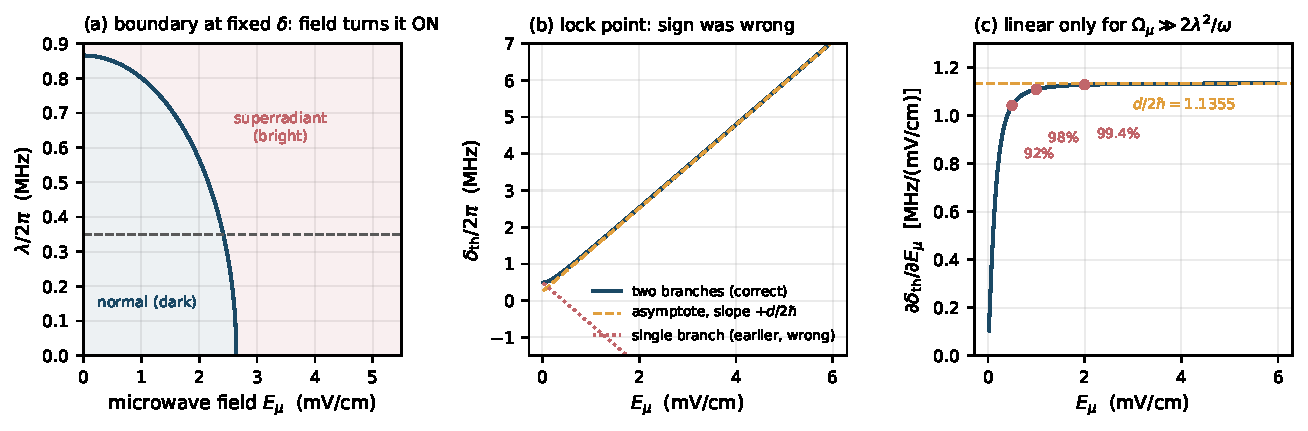
\includegraphics[width=\textwidth]{../figs/fig1_threshold.pdf}
  \caption{\textbf{The microwave field moves the phase boundary.}
  (a) Threshold coupling $\lc = \tfrac12\sqrt{\omega\,\Omu/2}$ versus microwave field for
  $\omega/2\pi = 1$~MHz, $\delta=0$ and the $53D_{5/2}\!\to\!54P_{3/2}$ dipole. At fixed
  $\lambda$ (dashed) the system crosses from superradiant to normal at a well-defined field.
  (b) Order parameter $\bar n$ at $\lambda/2\pi = 0.35$~MHz: the cavity goes dark above a
  critical field $E_\mu^c$. The steep square-root onset near $E_\mu^c$ is the transduction
  gain the scheme trades on.}
  \label{fig:threshold}
\end{figure}

The immediate observation is that the \emph{sign} of the response is the useful one: for
$\delta=0$ a \emph{larger} microwave field raises $\wt$ and hence $\lc$, extinguishing
superradiance. The sensor is therefore naturally operated as a bright-to-dark discriminator,
which is favourable for detection (one measures a decrease from a large signal, not an
increase from zero).

\section{Three read-out protocols}
\label{sec:protocols}

The construction supports three distinct protocols, with quite different characters. It is
worth separating them because most of the confusion in the critical-metrology literature
comes from conflating them.

\paragraph{Protocol A --- order-parameter read-out (analogue).}
Bias at fixed $\lambda$ slightly above threshold and monitor the emitted light. The signal
is $\partial\alpha/\partial\wt$, which diverges as $\mu\to1$:
\begin{equation}
  \frac{\partial \alpha}{\partial \wt}
  = \frac{\mu}{4\lambda\sqrt{1-\mu^2}} \xrightarrow[\ \mu\to1\ ]{} \infty .
\end{equation}
This is the direct analogue of what Ding \emph{et al.}~\cite{Ding2022} and Wang \emph{et
al.}~\cite{Wang2025} do with the Rydberg-interaction-driven critical point, and it is the
protocol most likely to be implemented first. Its weakness is that the divergent
susceptibility is not selective: laser intensity noise (which moves $\lambda$), cavity
length drift (which moves $\omega$) and stray dc fields (which move $\delta$) are amplified
by exactly the same factor as the signal.

\paragraph{Protocol B --- threshold (null) read-out.}
Hold $\lambda$ and $\omega$ fixed and servo the two-photon detuning $\delta$ so that the
system sits exactly at threshold. The lock point satisfies
\begin{equation}
  \delta_{\rm th} = \frac{4\lambda^2}{\omega} - \frac{\Omu}{2}
  \qquad\Longrightarrow\qquad
  \frac{\partial \delta_{\rm th}}{\partial E_\mu} = -\frac{d}{2\hbar},
\end{equation}
so a change in the microwave field is read out directly as a change in an \emph{optical
laser detuning}, which is a frequency and is therefore SI-traceable in exactly the sense
that makes Autler--Townes electrometry attractive~\cite{Sedlacek2012,Adams2023}. The scale
factor $d/2\hbar$ is the same as for Autler--Townes; what changes is the discriminant. In
AT electrometry the resolution is set by how well a splitting can be resolved against the
EIT linewidth. Here it is set by how sharply the threshold can be located, which is a
different --- and, near a continuous transition, potentially much steeper --- function.

To our reading of the literature this null variant has not been proposed, and it is the
most defensible original element of the idea. It also has a practical virtue: null methods
are first-order insensitive to gain calibration, which is precisely the weakness of
Protocol A.

\paragraph{Protocol C --- critical superheterodyne (recommended).}
Apply a microwave local oscillator with Rabi frequency $\Om_{\rm LO}$ to set the bias point
$\wt = \delta + \Om_{\rm LO}/2$ just below threshold, and let the weak signal field at
$\omega_{\rm LO}+\omega_{\rm IF}$ beat against it:
\begin{equation}
  \wt(t) = \delta + \frac{\Om_{\rm LO}}{2} + \frac{\Om_{\rm s}}{2}\cos(\omega_{\rm IF}t).
\end{equation}
The measurand is now a small \emph{modulation} of a Hamiltonian parameter, amplified by the
near-threshold susceptibility and detected at the intermediate frequency. This inherits the
linear-in-$E_{\rm s}$ scaling and technical-noise rejection that make the Rydberg
superheterodyne receiver~\cite{Jing2020} the most sensitive Rydberg electrometer built, and
adds critical gain on top. It is the configuration used for all the open-system numbers in
Sec.~\ref{sec:open}, and it is the one we would actually build.

\section{Metrological analysis}
\label{sec:metrology}

\subsection{Closed system: quantum Fisher information at criticality}

We first ask what the \emph{ground state} of Eq.~\eqref{eq:dicke} is worth as a probe of
$\wt$. Exact diagonalisation in the $j=N/2$ manifold (even-parity sector; photon cutoff
converged to $10^{-12}$, see Appendix~\ref{app:methods}) gives the quantum Fisher
information from the fidelity susceptibility,
$F_Q = 8\left(1-|\!\avg{\psi(\wt)|\psi(\wt+h)}\!|\right)/h^2$.

\begin{figure}[t]
  \centering
  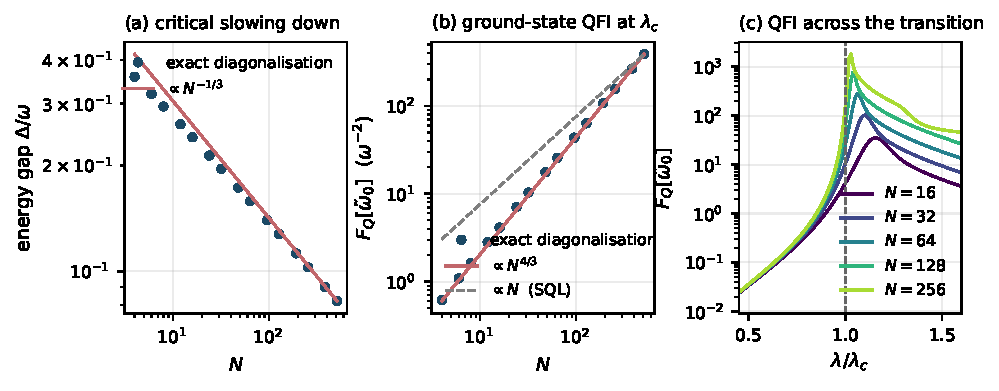
\includegraphics[width=\textwidth]{../figs/fig2_scaling.pdf}
  \caption{\textbf{Finite-size scaling at the critical point} ($\omega=\wt=1$,
  $\lambda=\lc$, $N \le 512$).
  (a) The energy gap closes as $N^{-1/3}$ (fitted $-0.317$ over $N\ge128$).
  (b) The quantum Fisher information for $\wt$ grows as $N^{4/3}$ (fitted $1.307$ over
  $N\ge128$), super-extensive and thus formally beyond the standard quantum limit
  $F_Q\propto N$ (dashed).
  (c) $F_Q$ across the transition; the peak sharpens and moves towards $\lambda_c$ as $N$
  grows.}
  \label{fig:scaling}
\end{figure}

Figure~\ref{fig:scaling} confirms the expected fully-connected-model
exponents~\cite{Garbe2022}: the gap closes as $N^{-1/3}$ and
\begin{equation}
  F_Q[\wt]\big|_{\lambda=\lc} \propto N^{4/3},
\end{equation}
with a fitted exponent of $1.307$ (asymptotic value $4/3 = 1.333$; the residual is the
expected slow finite-size correction, the fit drifting monotonically upward as the window
moves to larger $N$). In the normal phase we find, at $N=512$ and in the window
$N^{-2/3}\ll\varepsilon\ll1$,
\begin{equation}
  F_Q[\wt] \propto \varepsilon^{-2}, \qquad \varepsilon \equiv 1-\lambda^2/\lc^2,
\end{equation}
with a fitted exponent of $-2.0008$ --- the Gaussian critical scaling of a squeezed soft
mode, cut off at $\varepsilon_{\min}\sim N^{-2/3}$, which is exactly what produces the
$N^{4/3}$ peak.

\subsection{Why the $N^{4/3}$ is not free}

Taken at face value, $F_Q\propto N^{4/3}$ says $\delta\Omu \propto N^{-2/3}$, beating the
$N^{-1/2}$ standard quantum limit. This is the claim that critical-metrology proposals are
often built on, and it does not survive proper resource accounting. The gap closes as
$N^{-1/3}$, so adiabatic preparation of the critical ground state takes a time
$T_{\rm prep}\propto N^{1/3}$. Converting to a per-root-Hertz sensitivity,
\begin{equation}
  \delta\Omu\,\sqrt{T_{\rm prep}} \;\propto\; N^{-2/3}\cdot N^{1/6} \;=\; N^{-1/2},
\end{equation}
and the advantage cancels exactly. This is the content of Rams \emph{et
al.}~\cite{Rams2018}; Gietka \emph{et al.}~\cite{Gietka2021} show the cancellation survives
shortcuts to adiabaticity, and Gyhm \emph{et al.}~\cite{Gyhm2025} have recently established
a general $T^6$ ceiling on the quantum Fisher information of monotonic critical protocols.
A proposal built on the $N^{4/3}$ scaling alone would be building on sand, and this document
should not be used to write one.

The interesting question is therefore not the scaling but the \emph{prefactor}, which is
what the driven open system delivers.

\subsection{Open system: gain, bandwidth, squeezing and the input-referred floor}
\label{sec:open}

We linearise Eq.~\eqref{eq:dicke} in the normal phase (Holstein--Primakoff bosons $a$ for
the cavity, $b$ for the collective atomic mode), add cavity decay $\kappa$ and collective
decoherence $\gamma$, and drive the cavity coherently. In quadratures
$v=(x_a,p_a,x_b,p_b)$,
\begin{equation}
  \dot v = A v + f + B u, \qquad
  A = \begin{pmatrix}
    -\kappa & \omega & 0 & 0\\
    -\omega & -\kappa & -2\lambda & 0\\
    0 & 0 & -\gamma & \wt\\
    -2\lambda & 0 & -\wt & -\gamma
  \end{pmatrix},
\end{equation}
with vacuum inputs $u$. The measurand enters as $\delta H = \delta\wt\, b\dg b$, i.e.\ as a
coherent force
\begin{equation}
  s \;=\; \delta\wt\,\bigl(0,\,0,\,\bar p_b,\,-\bar x_b\bigr)
\end{equation}
proportional to the steady-state collective amplitude --- which is why Protocol~C needs the
probe drive. Output homodyne
spectra follow from $x_{\rm out} = \sqrt{2\kappa}\,x_a - x_{\rm in}$. The implementation is
validated by reproducing the exact vacuum level $S_{\rm out}=1/2$ for an empty cavity.

Throughout we use $\omega/2\pi = \wt/2\pi = 1$~MHz, $\kappa/2\pi = 50$~kHz and
$\gamma/2\pi=5$~kHz, giving a damped threshold $\lc/2\pi = 0.5006$~MHz.

\begin{figure}[t]
  \centering
  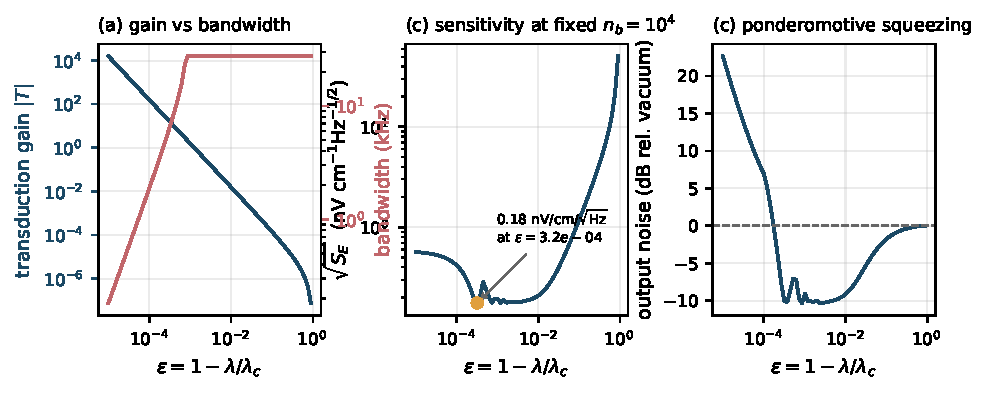
\includegraphics[width=\textwidth]{../figs/fig3_open.pdf}
  \caption{\textbf{Driven, damped sensor near threshold.}
  (a) Transduction gain (left axis) and response bandwidth (right axis) versus
  $\varepsilon = 1-\lambda/\lc$. At fixed collective occupation the gain grows as
  $\varepsilon^{-1}$ throughout, while the bandwidth stays pinned at $(\kappa+\gamma)/2 =
  27.5$~kHz until $\varepsilon\lesssim3\times10^{-4}$ and only then collapses as
  $\varepsilon^{+1}$. There is thus a window of \emph{free} gain before critical slowing
  down begins.
  (b) Quantum-noise-limited field sensitivity at fixed $n_b = 10^4$, with a broad optimum of
  $0.18~\mathrm{nV\,cm^{-1}Hz^{-1/2}}$.
  (c) The near-threshold system squeezes its own output by up to $10.3$~dB before atomic
  noise takes over.}
  \label{fig:open}
\end{figure}

Figure~\ref{fig:open} summarises the behaviour. Three points are worth stating precisely.

\paragraph{Gain and bandwidth.} At fixed collective occupation $n_b=\avg{b\dg b}$, the
transduction gain scales as $\varepsilon^{-1.000}$ over six decades. The bandwidth, however,
is \emph{not} immediately paid for: the slowest relaxation rate stays pinned at
$(\kappa+\gamma)/2 = 27.5$~kHz until $\varepsilon \lesssim 3\times10^{-4}$, below which the
soft mode becomes overdamped and the rate falls as $\varepsilon^{+1.002}$, giving a strict
gain--bandwidth product (constant to $0.78\%$). Practically: there is roughly three decades
of $\varepsilon$ over which criticality buys $10^3$ in gain at no bandwidth cost, and beyond
that it is a straight trade. This is a genuinely useful design statement and it does not
appear to have been made for this system.

\paragraph{Intrinsic squeezing.} Near threshold the soft mode is a degenerate parametric
amplifier and the output is squeezed --- we find up to $-10.3$~dB at
$\varepsilon\approx9\times10^{-4}$, degrading to excess noise once
$\varepsilon\lesssim10^{-4}$ where atomic decoherence dominates. The sensor generates its own
squeezed light; no external squeezed source is needed. This is a real, if modest,
quantum-enhancement channel and it is compatible with Protocol~C.

\paragraph{The control experiment that settles the matter.}
Sensitivity figures near a critical point are easy to inflate, because approaching threshold
increases the steady-state excitation as well as the gain. We therefore repeated the
calculation holding $n_b$ \emph{fixed} by re-solving for the drive at each $\varepsilon$.
The result is unambiguous:
\begin{equation}
  \boxed{\;\sqrt{S_{\wt}} \;=\; 0.72\,\sqrt{\gamma/n_b}\;}
  \label{eq:floor}
\end{equation}
with the numerical prefactor constant to one part in $10^4$ across five decades of $n_b$ and,
away from the extreme critical region, across three decades of $\varepsilon$. Equation
\eqref{eq:floor} is the standard quantum limit for $n_b$ atoms with coherence time
$1/\gamma$, up to a factor of order unity that we attribute to the intrinsic squeezing.

The physical reading: \textbf{criticality is a transducer, not a source of metrological
advantage}. It converts the atomic signal into a large optical signal --- which is exactly
what one needs to beat photodetector and technical noise, and is why Refs.~\cite{Ding2022,
Wang2025} report large Fisher-information gains --- but it does not lower the floor set by
how many atoms are coherently participating and for how long.

\subsection{Sensitivity in physical units}

Converting Eq.~\eqref{eq:floor} through $\delta\wt = \delta\Omu/2$ and $E_\mu=\hbar\Omu/d$:

\begin{table}[h]
\centering
\small
\begin{tabular}{lccc}
\toprule
Collective occupation $n_b$ & $\sqrt{S_{E}}$ (nV\,cm$^{-1}$Hz$^{-1/2}$) & SQL for $N=n_b$ & ratio \\
\midrule
$10^{3}$ & $0.567$ & $0.786$ & $0.72$\\
$10^{4}$ & $0.179$ & $0.248$ & $0.72$\\
$10^{5}$ & $0.057$ & $0.079$ & $0.72$\\
$10^{6}$ & $0.018$ & $0.025$ & $0.72$\\
$10^{7}$ & $0.0057$ & $0.0079$ & $0.72$\\
\bottomrule
\end{tabular}
\caption{Quantum-noise-limited field sensitivity at $\varepsilon=3\times10^{-3}$,
$\gamma/2\pi=5$~kHz. For reference: the Rydberg superheterodyne receiver of
Ref.~\cite{Jing2020} achieves $55~\mathrm{nV\,cm^{-1}Hz^{-1/2}}$; Ref.~\cite{Wang2025}
quotes $5.1~\mathrm{nV\,cm^{-1}Hz^{-1/2}}$ as the best sensitivity from conventional
SNR-enhancement methods, $49$--$50.3~\mathrm{nV\,cm^{-1}Hz^{-1/2}}$ for free-space critical
(non-equilibrium) electrometry, and $2.6~\mathrm{nV\,cm^{-1}Hz^{-1/2}}$ for its own
cavity-enhanced critical measurement.}
\end{table}

Two caveats attach to every number in that table. First, Holstein--Primakoff validity
requires $n_b \ll N$; taking $n_b/N \lesssim 10^{-2}$, the $n_b = 10^6$ row needs
$N\gtrsim10^{8}$ atoms coherently coupled to one cavity mode, which is demanding but not
absurd for a vapour cell and out of reach for a small cold cloud. Second, these are
\emph{quantum-noise-limited} figures with no allowance for Doppler broadening, transit-time
effects, inhomogeneous coupling across the cavity mode, laser frequency noise or dc-field
drift, all of which are what actually limits real Rydberg electrometers. Treat them as an
upper bound on what the mechanism can offer, not a prediction.

\section{Rydberg interactions: the link to the superradiant solid}
\label{sec:ising}

Reference~\cite{Zhang2013} is not the plain Dicke model: its content is what happens when
Rydberg--Rydberg interactions compete with the cavity coupling, producing a superradiant
\emph{solid} in which superradiance and crystalline order coexist, with first-order
boundaries. It is worth asking whether those interactions help or hurt the sensor.

Adding a nearest-neighbour Rydberg repulsion to Eq.~\eqref{eq:dicke},
\begin{equation}
  H_{\rm DI} = H + V\!\!\sum_{\avg{ij}} n_i n_j , \qquad n_i = S^z_i + \tfrac12 ,
\end{equation}
and taking a two-sublattice mean field on a bipartite lattice of coordination $z$ (with
$\alpha$ eliminated by its own stationarity condition),
\begin{equation}
  \frac{E}{N} = \omega\alpha^2 - \frac{\wt}{4}(\cos\theta_A+\cos\theta_B)
    + \lambda\alpha(\sin\theta_A+\sin\theta_B) + \frac{Vz}{2}n_A n_B,
  \qquad
  \alpha = -\frac{\lambda}{2\omega}(\sin\theta_A+\sin\theta_B),
\end{equation}
reproduces the phase structure of Ref.~\cite{Zhang2013}. We minimise this from $13\times13$
seeds per point with L-BFGS-B, and use adiabatic up/down sweeps in $\lambda$ as the
first-order diagnostic. Figure~\ref{fig:ising} shows the result, and it splits cleanly into
two regimes.

\begin{figure}[t]
  \centering
  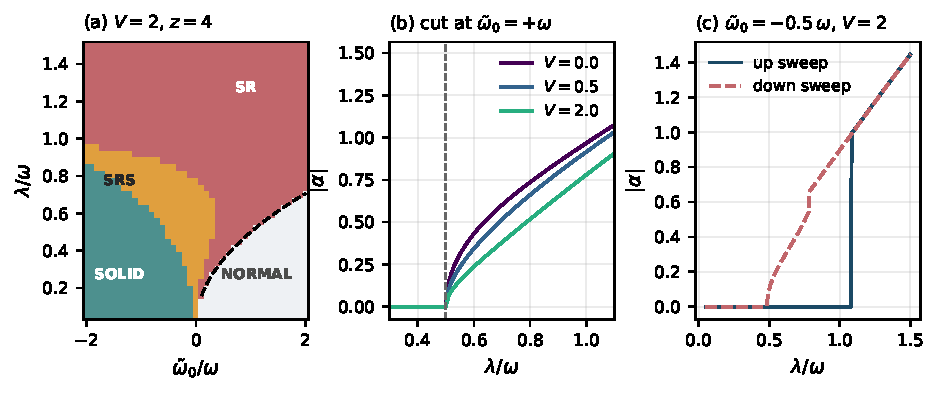
\includegraphics[width=\textwidth]{../figs/fig4_ising.pdf}
  \caption{\textbf{Rydberg interactions and the sensing threshold} ($V=2\omega$, $z=4$).
  (a) Mean-field phase diagram. The superradiant solid (SRS) of Ref.~\cite{Zhang2013} occupies
  only $\wt<0$; for $\wt>0$ --- the sensor's operating regime --- the boundary is the plain
  Dicke line $\lc=\tfrac12\sqrt{\omega\wt}$ (dashed), unmodified.
  (b) Cuts at $\wt=+\omega$ for $V=0,\,0.5,\,2$: the onset does not move, only the
  post-threshold amplitude is suppressed.
  (c) At $\wt=-0.5\,\omega$ the transition is strongly first order, with a hysteresis loop of
  height $0.985$ in $|\alpha|$.}
  \label{fig:ising}
\end{figure}

\paragraph{At the sensor's operating point, interactions are inert.} For $\wt>0$ the
normal-phase Rydberg population vanishes, so $n_A n_B \to 0$ and the interaction term does
nothing \emph{at} the transition. On a fine scan we find the onset at
$\lambda/\omega = 0.5005$ for every $V \in \{0,\,0.5,\,2,\,5\}$, i.e.\ no shift resolvable at
the $5\times10^{-4}$ level. Only the amplitude above threshold is suppressed
(Fig.~\ref{fig:ising}b). This is a genuinely useful robustness result: \emph{the calibration
curve Eq.~\eqref{eq:key} is immune to Rydberg interactions}, so atomic density fluctuations
--- which are exactly what moves the critical point in
Refs.~\cite{Ding2022,Wang2025} --- do not move it here. It is the sharpest technical argument
for preferring the Dicke critical point over the interaction-driven one.

\paragraph{The superradiant solid lives elsewhere, and it is first order.} The SOLID and SRS
phases appear only for $\wt<0$, i.e.\ when the dressed Rydberg level sits \emph{below}
$\ket{g}$ in the rotating frame (readily arranged by choosing $\delta<-\Omu/2$). There the
sequence on increasing $\lambda$ is SOLID $\to$ SRS $\to$ SR, and the transition is strongly
first order: up- and down-sweeps differ by $0.985$ in $|\alpha|$ at $\wt=-0.5\,\omega$,
$V=2\omega$.

The design conclusion, however, is largely independent of the details and is worth stating
now, because it runs against the intuition that "more Rydberg physics is better":

\begin{itemize}
  \item \textbf{For Protocols A and C, Rydberg interactions are a nuisance.} The clean
        collective enhancement of the Dicke model assumes $N$ independent emitters sharing
        one bright mode. Rydberg blockade caps the number of independently excitable atoms
        per blockade volume at one, so the effective $N$ entering $\lambda=g_0\sqrt{N}$ and
        the floor \eqref{eq:floor} is $N_{\rm eff} = V_{\rm mode}/V_{\rm blockade}$, not the
        atom number. Interactions also dephase the collective mode, raising $\gamma$. This
        is not a speculative worry: the quantum Monte Carlo study of
        Ref.~\cite{DickeIsing2025} reports exactly that, finding that Rydberg blockade
        significantly suppresses the cavity occupation.
        The sensor wants \emph{weak} interactions --- moderate $n$, or a Rydberg pair chosen
        for small van der Waals coefficient.
  \item \textbf{For a threshold detector, they are a feature.} If the transition is driven
        first order, the order parameter jumps discontinuously and the system latches, with
        hysteresis. That is useless for analogue metrology but excellent for a
        \emph{trigger}: a device that fires when the field crosses a settable level, with
        essentially unbounded gain at the switching point and built-in hysteresis to suppress
        chatter. This is a legitimate secondary application and it is the one place where
        Ref.~\cite{Zhang2013}'s first-order physics is directly useful.
\end{itemize}

Neither Ref.~\cite{Zhang2013} nor Ref.~\cite{DickeIsing2025} addresses sensing; both are
equilibrium phase-structure studies. What the sensing question adds is the observation
above --- that the calibration curve is interaction-immune at the operating point --- which
is the sharpest argument for preferring this critical point over the interaction-driven one.

\section{Prior art}
\label{sec:prior}

The relevant literature falls into four strands. The purpose of this section is to be
honest about how much of the idea is already occupied.

\subsection{Cavity-enhanced Rydberg electrometry --- the direct lineage}

Peng and co-workers have published a coherent programme along exactly this line.
Reference~\cite{Peng2018}, the seed paper, places a four-level Rydberg-EIT medium in a cavity
and reports a minimum detectable field roughly $8\times$ smaller than the cavity-free case
and a spectral resolution improved by more than $20\times$, attributing both to cavity
narrowing of the transmission features; it also notes robustness against control-field
amplitude and broadband tunability. The same group then moved to the collective regime:
Ref.~\cite{Yang2020} uses \emph{collective Rabi splitting}, obtaining a four-peak cavity
transmission whose outer splitting varies linearly with the microwave field, and reports
about $7\times$ improvement over plain EIT; Ref.~\cite{Wang2023} reports $196.7\times$ over
a bare atomic medium and $26.2\times$ over weak coupling, a minimum detectable strength of
$396.5~\mathrm{nV\,cm^{-1}}$ (a detection floor, not a per-root-hertz sensitivity), and
resolution gains of $216\times$ and $10\times$. Experimentally, Ref.~\cite{Liu2025}
demonstrates 18~dB of power-sensitivity enhancement using a microwave (not optical)
resonator, and Ref.~\cite{CavitySuperhet2025} demonstrates a cavity-enhanced Rydberg
\emph{superheterodyne} receiver with a 19~dB sensitivity gain.

\textbf{Implication for the idea.} The collective-coupling step is already taken. Anything
proposed here must be distinguished from ``$g_0\sqrt N$ in a cavity'', because
Ref.~\cite{Yang2020} is precisely that. The distinguishing feature has to be the
\emph{counter-rotating} terms and the phase transition they enable: on their published
abstracts, Refs.~\cite{Yang2020,Wang2023} are normal-phase Tavis--Cummings physics --- a
vacuum-Rabi/collective-Rabi splitting read out spectroscopically --- with no transition and
no critical point. Note this is exactly the same rotating-wave restriction found in
Ref.~\cite{Zhang2013} (Sec.~\ref{sec:ising}), so the counter-rotating terms are the single
ingredient that separates this proposal from the whole of that lineage.

\subsection{Critical Rydberg metrology --- the closest competitor}

Ding, Liu, Shi, Guo, M\o{}lmer and Adams~\cite{Ding2022} demonstrated many-body enhanced
microwave metrology at the critical point of a non-equilibrium Rydberg gas, reporting a
Fisher information three orders of magnitude above the independent-particle value and an
equivalent sensitivity of $49~\mathrm{nV\,cm^{-1}Hz^{-1/2}}$. Wang, Liang, Wang and
co-workers~\cite{Wang2025} then put that critical system inside an optical cavity, reporting
more than two orders of magnitude of additional Fisher information and
$2.6~\mathrm{nV\,cm^{-1}Hz^{-1/2}}$.

Both papers were read in full, and the mechanism is unambiguous. The critical point is that
of a \emph{non-equilibrium phase transition} (NEPT) --- the optical bistability of a
laser-driven Rydberg ensemble, arising from the competition between long-range Rydberg
interactions, drive strength and dissipation. The ``critical point'' is operationally the
coupling-laser frequency at which the transmission jumps, the jump direction depends on the
scan direction, and a hysteresis loop is observed. Reference~\cite{Wang2025} works in a hot
caesium vapour cell ($6S_{1/2}\!\to\!6P_{3/2}\!\to\!47D_{5/2}$, microwave to $48P_{3/2}$),
uses the sharp bistability edge as a frequency discriminator, and quantifies it with the
\emph{classical} Fisher information; the cavity's role is to steepen that edge (by
$>10\times$ in slope, $>100\times$ in Fisher information). No light--matter phase transition
is involved anywhere in either work.

\textbf{This is the strongest prior art and it must be addressed head-on.}
Reference~\cite{Wang2025} is ``critical Rydberg metrology in a cavity'', which is a fair
one-line summary of the present idea too. The substantive difference is \emph{which}
criticality:
\begin{itemize}
  \item Refs.~\cite{Ding2022,Wang2025} use the \emph{dissipative, Rydberg-interaction-driven}
        phase transition (optical bistability of the driven Rydberg ensemble). Its critical
        point is set by atomic density and interaction strength, and therefore drifts with
        temperature, density and stray fields, and cannot be tuned quickly. It is also
        hysteretic, so the discriminator is scan-direction dependent.
  \item The present proposal uses the \emph{light--matter} (Dicke) transition. Its critical
        point is set by $\lambda \propto$ laser amplitude and by $\omega$, both of which are
        tunable in situ on microsecond timescales and can be servoed. The critical point
        is a controlled instrument setting rather than a property of the sample.
\end{itemize}
That difference is real and is worth a paper, but it is a difference of \emph{controllability
and traceability}, not of sensitivity scaling. Claiming the latter would be wrong (see
Sec.~\ref{sec:open}).

\subsection{Critical quantum metrology --- the theory that constrains the claims}

Garbe \emph{et al.}~\cite{Garbe2020} established the finite-component critical metrology
paradigm with the quantum Rabi model, and Ref.~\cite{Garbe2022} worked out the
fully-connected-model scaling (static, quench and finite-time-ramp protocols, including
Kibble--Zurek scaling) whose exponents we reproduce in Fig.~\ref{fig:scaling}. Against these,
Rams \emph{et al.}~\cite{Rams2018}, Gietka \emph{et al.}~\cite{Gietka2021,Gietka2022} and
Gyhm \emph{et al.}~\cite{Gyhm2025} constrain what can be claimed once time is counted as a
resource. Any write-up of this idea must engage with that second group of references
explicitly; a referee will otherwise do it for you.

\subsection{Dicke-model engineering and Rydberg cavity QED --- the feasibility base}

The engineered Dicke model is experimentally established: proposed by Dimer \emph{et
al.}~\cite{Dimer2007}, realised by Baden \emph{et al.}~\cite{Baden2014} with cavity-assisted
Raman transitions, and separately by Baumann \emph{et al.}~\cite{Baumann2010} via
self-organisation of a BEC. For the Rydberg platform specifically,
Ref.~\cite{Anisotropic2025} gives a periodic-driving recipe for the anisotropic Dicke model
in a cavity-coupled Rydberg array with a counter-rotating/rotating ratio tunable from zero
to infinity, and Ref.~\cite{DickeIsing2025} maps the resulting phase diagram by quantum
Monte Carlo. The enabling theory is therefore in place; what is missing is the sensing
application. Cavity Rydberg polaritons have been observed~\cite{Ningyuan2016},
including the suppression of inhomogeneous broadening by collective strong coupling that this
proposal needs. On the sensing side, Rydberg electrometers now approach the standard quantum
limit in cold atoms~\cite{SciAdv2024} and reach within 1.0~dB of it in tweezer
arrays~\cite{PRL2026}, and collective-radiative linewidth engineering for Rydberg microwave
sensing has just been proposed~\cite{PRA2026}. Rydberg systems can also be spin-squeezed
directly~\cite{Bloqade2023}, which is the main competing route to sub-SQL electrometry.

\subsection{What appears to be unoccupied}

An arXiv full-text search (queries combining \emph{Dicke}/\emph{superradiant} with
\emph{Rydberg}, \emph{electrometry}, \emph{microwave electric field}, \emph{metrology} and
\emph{sensing}) returns no hit that uses the light--matter superradiant transition as the
sensing element for microwave electrometry: the Dicke$+$Rydberg literature
(Refs.~\cite{Zhang2013,Anisotropic2025,DickeIsing2025} and the Rydberg-dressed open-Dicke
study of Ref.~\cite{RydDressed2026}) is uniformly concerned with phase structure and
dynamics, and the critical-electrometry literature is uniformly concerned with the
interaction-driven NEPT. On that basis:

\begin{enumerate}
  \item \textbf{Unoccupied.} Using the \emph{Dicke} (light--matter) superradiant transition,
        rather than a Rydberg-interaction transition, as the critical resource for microwave
        electrometry --- together with the observation of Sec.~\ref{sec:ising} that this
        makes the calibration curve immune to Rydberg interactions and to atomic density.
  \item \textbf{Unoccupied, but with near neighbours.} The null / threshold-crossing read-out
        of Protocol~B. The general idea of biasing at a dynamical threshold and reading out a
        frequency is not new: Ref.~\cite{InjPull2026} pulls a self-sustained microwave
        oscillator through its Adler synchronisation boundary and reports enhanced
        sensitivity near synchronisation, and Ref.~\cite{Ramsey2023} exploits a sub- to
        superradiant emission threshold for atomic state read-out. What is not in the
        literature is the specific realisation here, in which the measurand is the
        \emph{optical two-photon detuning required to hold a light--matter phase transition
        at threshold}. The novelty claim should be worded at that level of specificity, not
        as ``threshold-based sensing''.
  \item \textbf{Unoccupied, and useful.} The explicit gain--bandwidth characterisation of a
        critical Rydberg sensor, including the finding that there is a wide window of gain
        before critical slowing down is paid for.
\end{enumerate}

Items 1 and 3 are the safest. Item 2 is the most interesting but needs the careful wording
above.

\section{Assessment}
\label{sec:verdict}

\subsection{Is it a good idea?}

\textbf{Yes, with one large caveat about how it is framed.} The physics is sound, the
mapping from measurand to critical point is exact and simple, the required experimental
ingredients all exist separately, and the numbers are competitive. But the natural framing
--- ``criticality gives super-classical scaling for electrometry'' --- is not supportable,
and Eq.~\eqref{eq:floor} shows why in this specific system rather than by appeal to general
theorems. The idea should be framed as \emph{a tunable, SI-traceable critical amplifier for
Rydberg electrometry}, and it is a good idea under that framing.

\subsection{Benefits}

\begin{itemize}
  \item \textbf{Transduction gain where it is needed.} $\varepsilon^{-1}$ gain, with roughly
        three decades of it free of bandwidth cost. Real Rydberg sensors are usually limited
        by optical detection and technical noise, not by atomic projection noise, so gain at
        the atomic stage is directly valuable.
  \item \textbf{In-situ tunable critical point.} Unlike the density-driven critical point of
        Refs.~\cite{Ding2022,Wang2025}, $\lc$ here is set by laser power and can be servoed,
        making the operating point stable and reproducible.
  \item \textbf{SI traceability via Protocol B.} Reading the measurand as a laser detuning
        preserves the metrological virtue that makes Rydberg electrometry attractive to
        national metrology institutes.
  \item \textbf{Self-generated squeezing.} Up to $10$~dB, with no external squeezed source
        and no separate entanglement-generation step.
  \item \textbf{Bright-to-dark operation.} The response sign is favourable for detection.
  \item \textbf{A trigger mode.} With strong Rydberg interactions the transition can be made
        first order, giving a latching threshold detector.
\end{itemize}

\subsection{Risks and objections}

\begin{itemize}
  \item \textbf{The scaling advantage is illusory.} Established in Sec.~\ref{sec:open} and
        by Refs.~\cite{Rams2018,Gietka2021,Gyhm2025}. This is the objection a referee will
        raise first.
  \item \textbf{Criticality amplifies drift as well as signal.} Protocol A has no
        discrimination between $\delta\wt$ from the microwave field and $\delta\lambda$ from
        laser intensity noise or $\delta\omega$ from cavity drift --- formally, the critical
        QFI matrix is sloppy~\cite{MultiCrit2026}. Protocol C's IF encoding and Protocol B's
        null lock are the mitigations, and they are not optional.
  \item \textbf{Bandwidth.} $27.5$~kHz at the parameters used, set by $(\kappa+\gamma)/2$.
        That is fine for metrology and useless for a communications receiver. A higher-$\kappa$
        cavity trades gain for bandwidth in the usual way.
  \item \textbf{Rydberg blockade caps $N_{\rm eff}$}, which is what Eq.~\eqref{eq:floor}
        actually depends on. This is in direct tension with the Ref.~\cite{Zhang2013} physics,
        which \emph{wants} strong interactions.
  \item \textbf{Engineering overhead.} Two Raman channels plus a high-finesse cavity plus
        (probably) cold atoms is a substantial step away from the vapour-cell simplicity that
        makes Rydberg electrometry commercially interesting --- though less of a step than it
        was, given Refs.~\cite{Anisotropic2025,CavitySuperhet2025}.
  \item \textbf{Decoherence cuts off the critical scaling.} The divergence is truncated once
        the soft-mode frequency falls below $\gamma$, i.e.\ at
        $\varepsilon_{\min}\sim(\gamma/\omega)^2$; with vapour-cell linewidths this bites
        early.
  \item \textbf{Prior art is close.} Reference~\cite{Wang2025} in particular will be cited
        against any claim of novelty that is not carefully worded.
\end{itemize}

\subsection{Recommended programme}

\begin{enumerate}
  \item \textbf{Theory paper, correctly framed.} Title along the lines of ``Critical Dicke
        amplification for SI-traceable Rydberg electrometry''. Lead with Protocol~B (null
        read-out) as the novel element and the gain--bandwidth analysis as the practical one.
        State the no-go results up front rather than being caught by them.
  \item \textbf{Do the calculation the referee will ask for.} A full Ziv--Zakai or Bayesian
        treatment of Protocol~B's threshold-location precision, since the Cramér--Rao bound is
        the wrong tool for a null measurement, and a proper account of inhomogeneous coupling
        across the cavity mode.
  \item \textbf{The obvious precursor experiment is already done.} Protocol~C in the
        \emph{Tavis--Cummings} regime (no counter-rotating terms, no phase transition)
        is a cavity-enhanced Rydberg superheterodyne receiver, and
        Ref.~\cite{CavitySuperhet2025} has demonstrated exactly that, with a 19~dB
        sensitivity gain. That removes the de-risking step from the critical path: the
        apparatus exists and the gain mechanism is confirmed. Go straight to adding the
        counter-rotating channel, following Ref.~\cite{Anisotropic2025}.
  \item \textbf{Address the selectivity objection formally.} The complaint that criticality
        amplifies $\delta\lambda$ and $\delta\omega$ as readily as $\delta\wt$ is, in
        estimation language, the statement that the critical QFI matrix is sloppy.
        Reference~\cite{MultiCrit2026} shows for the Dicke model that multi-parameter
        critical estimation can retain divergent precision at the cost of a reduced scaling
        exponent, and that a Dicke dimer with photon hopping restores the optimal scaling.
        That is the right framework in which to answer the objection rather than to concede
        it.
\end{enumerate}

\appendix

\section{Numerical methods}
\label{app:methods}

All code is in \texttt{code/}; all figures are regenerated by \texttt{code/make\_figs.py}.

\paragraph{Exact diagonalisation.} Equation~\eqref{eq:dicke} is built on the product of the
$j=N/2$ spin manifold ($N+1$ states) and a truncated Fock space. Since
$\partial H/\partial\wt = J_z$ is parity-even, only the even-parity sector contributes to
$F_Q$ and the calculation is restricted to it, which also removes the closing odd-parity gap
from the eigensolver's path. Photon truncation was verified at $N=200$, $\lambda=\lc$:
$F_Q$ agrees to twelve digits between $n_{\max}=60$ and $n_{\max}=120$; production runs used
$n_{\max}=100$--$140$. The QFI is obtained from the fidelity susceptibility with a symmetric
step $h = 10^{-4}\wt$.

\paragraph{Quantum Langevin.} The linearised open-system calculation uses symmetrised
two-sided spectra with vacuum inputs, diffusion matrix $D=\mathrm{diag}(\kappa,\kappa,
\gamma,\gamma)$, and the input--output relation $x_{\rm out}=\sqrt{2\kappa}x_a - x_{\rm in}$
including the cross-correlation between intracavity field and input vacuum. The
implementation returns exactly $S_{\rm out}=1/2$ for an empty cavity, which fixes all
normalisation conventions. The damped threshold $\lc$ is located by bisection on
$\max\mathrm{Re}\,\mathrm{eig}(A)=0$. Homodyne angles are optimised on a $361$-point grid.

\paragraph{Parameters.} Unless stated: $\omega/2\pi=\wt/2\pi=1$~MHz, $\kappa/2\pi=50$~kHz,
$\gamma/2\pi=5$~kHz, $d=1774.82\,ea_0$ for $^{87}$Rb $53D_{5/2}\!\to\!54P_{3/2}$.

\begin{thebibliography}{99}
\small

\bibitem{Peng2018} Y.~Peng, J.~Wang, A.~Yang, Z.~Jia, D.~Li, and B.~Chen,
  \emph{Cavity-enhanced microwave electric field measurement using Rydberg atoms},
  J.~Opt.~Soc.~Am.~B \textbf{35}, 2272 (2018).
  \href{https://doi.org/10.1364/JOSAB.35.002272}{doi:10.1364/JOSAB.35.002272}.

\bibitem{Zhang2013} X.-F.~Zhang, Q.~Sun, Y.-C.~Wen, W.-M.~Liu, S.~Eggert, and A.-C.~Ji,
  \emph{Rydberg polaritons in a cavity: a superradiant solid},
  Phys.~Rev.~Lett.~\textbf{110}, 090402 (2013); arXiv:1207.4238.
  \href{https://doi.org/10.1103/PhysRevLett.110.090402}{doi:10.1103/PhysRevLett.110.090402}.

\bibitem{Yang2020} A.~Yang, W.~Zhou, S.~Zhao, Y.~Xu, F.~Jelezko, Y.~Li, and Y.~Peng,
  \emph{Enhanced measurement of microwave electric fields with collective Rabi splitting},
  J.~Opt.~Soc.~Am.~B \textbf{37}, 1664 (2020).

\bibitem{Wang2023} Y.~Wang, Z.~Jia, Y.~Yu, B.~Chen, and Y.~Peng,
  \emph{Rydberg-atom-based measurements of microwave electric fields with cavity quantum
  electrodynamics}, J.~Opt.~Soc.~Am.~B \textbf{40}, 2604 (2023).

\bibitem{Liu2025} \emph{Cavity-enhanced Rydberg atom microwave receiver},
  Chin.~Phys.~Lett.~\textbf{42}, 053201 (2025); arXiv:2404.06915.

\bibitem{Ding2022} D.-S.~Ding, Z.-K.~Liu, B.-S.~Shi, G.-C.~Guo, K.~M\o{}lmer, and
  C.~S.~Adams, \emph{Enhanced metrology at the critical point of a many-body Rydberg atomic
  system}, Nat.~Phys.~\textbf{18}, 1447 (2022); arXiv:2207.11947.

\bibitem{Wang2025} Q.~Wang, Y.~Liang, Z.~Wang, \emph{et al.},
  \emph{High-precision measurement of microwave electric field by cavity-enhanced critical
  behavior in a many-body Rydberg atomic system},
  Sci.~China Phys.~Mech.~Astron.\ (2025); arXiv:2502.19761.
  \href{https://doi.org/10.1007/s11433-024-2622-x}{doi:10.1007/s11433-024-2622-x}.

\bibitem{Jing2020} M.~Jing, Y.~Hu, J.~Ma, H.~Zhang, L.~Zhang, L.~Xiao, and S.~Jia,
  \emph{Atomic superheterodyne receiver based on microwave-dressed Rydberg spectroscopy},
  Nat.~Phys.~\textbf{16}, 911 (2020); arXiv:1902.11063.

\bibitem{Sedlacek2012} J.~A.~Sedlacek, A.~Schwettmann, H.~K\"ubler, R.~L\"ow, T.~Pfau, and
  J.~P.~Shaffer, \emph{Microwave electrometry with Rydberg atoms in a vapour cell using
  bright atomic resonances}, Nat.~Phys.~\textbf{8}, 819 (2012).

\bibitem{Adams2023} \emph{Quantum sensing of microwave electric fields based on Rydberg
  atoms}, Rep.~Prog.~Phys.\ (2023).
  \href{https://doi.org/10.1088/1361-6633/acf22f}{doi:10.1088/1361-6633/acf22f}.

\bibitem{Dimer2007} F.~Dimer, B.~Estienne, A.~S.~Parkins, and H.~J.~Carmichael,
  \emph{Proposed realization of the Dicke-model quantum phase transition in an optical cavity
  QED system}, Phys.~Rev.~A \textbf{75}, 013804 (2007).

\bibitem{Baden2014} M.~P.~Baden, K.~J.~Arnold, A.~L.~Grimsmo, S.~Parkins, and M.~D.~Barrett,
  \emph{Realization of the Dicke model using cavity-assisted Raman transitions},
  Phys.~Rev.~Lett.~\textbf{113}, 020408 (2014); erratum \textbf{118}, 199901 (2017).

\bibitem{Baumann2010} K.~Baumann, C.~Guerlin, F.~Brennecke, and T.~Esslinger,
  \emph{Dicke quantum phase transition with a superfluid gas in an optical cavity},
  Nature \textbf{464}, 1301 (2010).

\bibitem{Emary2003} C.~Emary and T.~Brandes,
  \emph{Chaos and the quantum phase transition in the Dicke model},
  Phys.~Rev.~E \textbf{67}, 066203 (2003).

\bibitem{Rzazewski1975} K.~Rz\k{a}\.zewski, K.~W\'odkiewicz, and W.~\.Zakowicz,
  \emph{Phase transitions, two-level atoms, and the $A^2$ term},
  Phys.~Rev.~Lett.~\textbf{35}, 432 (1975).

\bibitem{Nataf2010} P.~Nataf and C.~Ciuti,
  \emph{No-go theorem for superradiant quantum phase transitions in cavity QED and counterexample
  in circuit QED}, Nat.~Commun.~\textbf{1}, 72 (2010).

\bibitem{Garbe2020} L.~Garbe, M.~Bina, A.~Keller, M.~G.~A.~Paris, and S.~Felicetti,
  \emph{Critical quantum metrology with a finite-component quantum phase transition},
  Phys.~Rev.~Lett.~\textbf{124}, 120504 (2020).

\bibitem{Garbe2022} L.~Garbe, O.~Abah, S.~Felicetti, and R.~Puebla,
  \emph{Critical quantum metrology with fully-connected models: from Heisenberg to
  Kibble--Zurek scaling}, Quantum Sci.~Technol.~\textbf{7}, 035010 (2022); arXiv:2110.04144.

\bibitem{Rams2018} M.~M.~Rams, P.~Sierant, O.~Dutta, P.~Horodecki, and J.~Zakrzewski,
  \emph{At the limits of criticality-based quantum metrology: apparent super-Heisenberg
  scaling revisited}, Phys.~Rev.~X \textbf{8}, 021022 (2018); arXiv:1702.05660.

\bibitem{Gietka2021} K.~Gietka, F.~Metz, T.~Keller, and J.~Li,
  \emph{Adiabatic critical quantum metrology cannot reach the Heisenberg limit even when
  shortcuts to adiabaticity are applied}, Quantum \textbf{5}, 489 (2021); arXiv:2103.12939.

\bibitem{Gietka2022} K.~Gietka, L.~Ruks, and T.~Busch,
  \emph{Understanding and improving critical metrology: quenching superradiant light--matter
  systems beyond the critical point}, Quantum \textbf{6}, 700 (2022); arXiv:2110.04048.

\bibitem{Gyhm2025} J.-Y.~Gyhm, H.~Kwon, and M.-J.~Hwang,
  \emph{Fundamental scaling limit in critical quantum metrology}, arXiv:2506.19003 (2025).

\bibitem{Ningyuan2016} J.~Ningyuan, A.~Georgakopoulos, A.~Ryou, N.~Schine, A.~Sommer, and
  J.~Simon, \emph{Observation of cavity Rydberg polaritons},
  Phys.~Rev.~A \textbf{93}, 041802(R) (2016); arXiv:1511.01872.

\bibitem{SciAdv2024} \emph{Approaching the standard quantum limit of a Rydberg-atom microwave
  electrometer}, Sci.~Adv.\ (2024).
  \href{https://doi.org/10.1126/sciadv.ads0683}{doi:10.1126/sciadv.ads0683}.

\bibitem{PRL2026} \emph{Microwave electrometry with quantum-limited resolutions in a
  Rydberg-atom array}, Phys.~Rev.~Lett.\ (2026); arXiv:2512.05413.

\bibitem{PRA2026} \emph{Superradiant and subradiant linewidth engineering for
  quantum-enhanced microwave sensing with Rydberg atoms}, Phys.~Rev.~A (2026).

\bibitem{Bloqade2023} G.~Bornet \emph{et al.},
  \emph{Scalable spin squeezing in a dipolar Rydberg atom array},
  Nature \textbf{621}, 728 (2023); arXiv:2303.08053.

\bibitem{DickeIsing2025} \emph{Quantum phase transitions of the anisotropic Dicke--Ising model
  in driven Rydberg arrays}, Phys.~Rev.~A (2026); arXiv:2511.22230.

\bibitem{Anisotropic2025} \emph{Engineering anisotropic Dicke model with dipole-dipole
  interaction for Rydberg atom arrays in cavity}, arXiv:2503.13949 (2025).

\bibitem{CavitySuperhet2025} \emph{Cavity-enhanced Rydberg atomic superheterodyne receiver},
  arXiv:2502.20792 (2025).

\bibitem{MultiCrit2026} \emph{Multi-parameter multi-critical metrology of the Dicke model},
  arXiv:2603.03451 (2026).

\bibitem{InjPull2026} \emph{Microwave power-to-frequency transduction via injection pulling
  of a self-sustained oscillator for Rydberg superheterodyne sensing}, arXiv:2605.08535 (2026).

\bibitem{Ramsey2023} \emph{Collectively enhanced Ramsey readout by cavity sub- to
  superradiant transition}, arXiv:2306.12544 (2023).

\bibitem{RydDressed2026} \emph{Dissipative dynamics and superradiant continuous time crystal
  in a Rydberg-dressed Dicke system}, arXiv:2604.18119 (2026).

\end{thebibliography}

\end{document}
